\documentclass[conference,draftcls,onecolumn]{IEEEtran}


\usepackage[utf8]{inputenc}
\usepackage[linesnumbered,lined, algoruled]{algorithm2e}
\usepackage{algorithmic}
\usepackage{amsmath}
\usepackage{amsthm}
\usepackage{amsfonts}
\usepackage{amssymb}
\usepackage{balance}
\usepackage{bm}
\usepackage{color,soul}
%\usepackage{epstopdf}
\usepackage[acronym,shortcuts]{glossaries}
\usepackage{graphicx}
\usepackage{graphics}
%\usepackage[inline]{enumitem}
\makeglossaries
%%% Glossaries/Acronyms


\newacronym{auc}{AUC}{area under the curve}
\newacronym{bs}{AP}{access point}
\newacronym{ce}{CE}{cross entropy}
\newacronym{cdf}{CDF}{cumulative distribution function}
\newacronym{fa}{FA}{false alarm}
\newacronym{kl}{K-L}{Kullback-Leibler}
\newacronym{ls}{LS}{least-squares}
\newacronym{llr}{LLR}{log likelihood-ratio}
\newacronym{los}{LOS}{line of sight}
\newacronym{lssvm}{LS-SVM}{least squares SVM}
\newacronym{md}{MD}{mis-detection}
\newacronym{ml}{ML}{machine learning}
\newacronym{mlp}{MLP}{multy-layer perceptron}
\newacronym{mse}{MSE}{mean squared error}
\newacronym[\glslongpluralkey={neural networks}]{nn}{NN}{neural network}
\newacronym{np}{N-P}{Neyman-Pearson}
\newacronym{oclssvm}{OCLSSVM}{one-class least-square \ac{svm}}
\newacronym{pdf}{PDF}{probability density function}
\newacronym{pmd}{PMD}{probability mass distribution}
\newacronym{pso}{PSO}{particle swarm optimization}
\newacronym{rnn}{RNN}{replicator neural network}
\newacronym{roc}{ROC}{receiver operating characteristic}
\newacronym{roi}{ROI}{region of interest}
\newacronym{rss}{RSS}{received signal strength}
\newacronym[\glslongpluralkey={support vector machines}]{svm}{SVM}{support vector machine}
\newacronym{ue}{UE}{user equipment}
\newacronym{wsn}{WSN}{wireless sensor network}
\newacronym{irlv}{IRLV}{in-region location verification}

\newcommand{\cross}[2]{H_{#1}(#2)}
\newcommand{\hatcross}[2]{\hat{H}_{#1}(#2)}
\newcommand{\gy}{g(\bm y)}
\newcommand{\E}[2]{\mathbb{E}_{#1}\left[#2\right]}
\newcommand{\pr}[1]{\mathbb{P} \left[ #1 \right]}

\newtheorem{theorem}{Theorem}

%\usepackage[autostyle]{csquotes}
\usepackage[backend=biber,style=ieee]{biblatex}
\bibliography{bibliography2.bib}


\title{Location-Verification and Network Planning \\ via Machine Learning Approaches}
\author{Alessandro Brighente, Francesco Formaggio, Marco Centenaro, Giorgio Maria Di Nunzio, and    Stefano Tomasin \\ {\small Department of Information Engineering, University of Padova, via G. Gradenigo 6/B, Padova, Italy. first.lastname@dei.unipd.it} }
\date{today}

\begin{document}

\maketitle

\begin{abstract}
For a \ac{ue} transmitting over a wireless network we consider the \ac{irlv} problem of deciding if the \ac{ue} is inside or outside a specific physical area (e.g., a safe room). The decision process exploits the features of the channel between the \ac{ue} and a set of network \acp{bs}. A  \ac{ml} approach is used, based on a \ac{nn}. The \ac{nn} is trained with the channel features (in particular, noisy attenuation values) collected by the \acp{bs} for various positions both inside and outside the specific area and outputs a decision between the \ac{ue} being inside or outside the area. By seeing the \ac{irlv} problem as an hypothesis testing problem, we address the optimal positioning of the \acp{bs} for minimizing either the \ac{auc} of the \ac{roc} or  the \ac{ce} between the \ac{nn} output and the true user position set. In order to solve the minimization problem we propose a two-stage \ac{pso} algorithm. We show that for a long training and a \ac{nn} with enough neurons the proposed solution achieves the performance of the \ac{np} lemma.
\end{abstract}

\begin{IEEEkeywords}
Physical layer security, location verification, neural network, network planning.
\end{IEEEkeywords}
\glsresetall

\section{Introduction}

Applications using information on the user location are rapidly spreading, also to ensure that some services are obtained only in pre-determined areas. For example, some on line gambling sites can be used only when in the state where the site is registered.

In order to establish the user position we can rely on the reports of localization modules in the user device, e.g., the GPS module. However, tempering with devices or on the software interface to the GPS module is relatively easy \cite{ceccato2018exploiting}. Thus more reliable solutions must be explored.

Location verification systems aim at verifying the position of devices in sensor networks \cite{Zeng-survey, 8376254}, Internet of Things \cite{7903611}, and mobile cell networks \cite{quaglia}. Various approaches have been proposed for location verification, typically based on the measurement of the distance between the transmitter and other users  or  anchor nodes belonging to the network infrastructure. The distance measures are obtained, for example, through the \ac{rss} at anchor nodes for signals transmitted by the terminal under verification.  This problem is closely related to the {\em user authentication} at the physical layer, where wireless channel features are exploited to verify the sender of a message \cite{7270404}.

We focus here on  \ac{irlv}, i.e., the problem of deciding whether a message coming from a terminal over a wireless network has been originated from a specific physical area, e.g., a safe room, or not \cite{Zeng-survey}. \ac{irlv} can be seen as an hypothesis testing problem between two alternatives, namely being inside or outside the specific area. Among proposed solutions, we recall distance bounding techniques with rapid exchanges of packets between the verifier and the prover \cite{Brands}, also using radio-frequency and ultrasound signals \cite{Sastry}, and solutions based on the use of anchor nodes and increasing transmit power by the sender \cite{Vora}. More recently, a delay-based verification technique has been proposed  in \cite{7145434}, leveraging geometric properties of triangles, which prevents an adversary from manipulating measured delays. 

In this paper, we consider the \ac{irlv} problem for a \ac{ue} connected to a set of network \acp{bs}. The decision on the user position is taken on the basis of observed features of the channel over which communication occurs. For exemplary purposes we focus here on the observation of the attenuation of the channel between the \ac{ue} and the \acp{bs}. We first observe that the  \ac{np} lemma \cite{Neyman289} is the optimal solution to \ac{irlv} by providing the hypothesis test with the minimum \ac{md} probability for a given \ac{fa} probability.
Note that in the \ac{irlv} literature there is no detailed \ac{fa}-\ac{md} analysis nor a clear comparison with the optimal \ac{np} solution.
 However, \ac{np}  requires the explicit knowledge of the statistics of the observed features, which may not always be available. Therefore we propose a \ac{ml} approach  where i) first channel measurements are collected by trusted nodes both inside and outside the \ac{roi}, ii) then a machine is trained to take decisions between the two hypotheses, iii) the machine is exploited to take decisions on the unknown \acp{ue}. \ac{ml} techniques have already found application in user authentication (see  \cite{xiao-2018} and references therein). However, \ac{ml} solutions have never been applied before to \ac{irlv}, to the best of authors' knowledge. 

Then, leveraging \ac{irlv} solution we address the problem of optimum positioning of the \acp{bs} (network planning). Two metrics are considered fo this optimization: the \ac{ce} of \ac{nn} training, and the \ac{auc} of the \ac{roc}. We propose a two-stage \ac{pso} algorithm minimizing either the \ac{ce} or the \ac{roc} \ac{auc}. Simulation results of the proposed solution over channels with shadow fading complete this work.

%The rest of the paper is organized as follows. In Section \ref{sec:sys model} we describe the system and channel model. Section \ref{sec: ml} describes the optimal \ac{np} solution and the \ac{ml} solution to \ac{irlv}. In Section \ref{sec:bsPos} we discuss the \acp{bs} positioning problem and we show how \ac{ml} can be used to solve it. In Section \ref{sec: nr} we present numerical results showing the effectiveness of the proposed solutions for both \ac{irlv} and \ac{bs} positioning, before conclusions outlined in Section \ref{sec:conc}.

%Network planning, i.e., designing optimal \acp{bs}' layout maximizing a chosen metric, has been studied in the literature in the context of \ac{wsn} \cite{bogdanov2004power} \cite{akkaya2007positioning} and cellular systems \cite{mathar2001optimal} \cite{glasser2005complexity}  \cite{islam2012capacity} \cite{yangyang2004particle}. In \cite{bogdanov2004power} the sensors network is optimized using as metric the rate of transmission between nodes. The resulting optimization is then solved using two heuristic iterative algorithms, since the problem is NP-complete. For a comparison between other proposed approaches and metric choices for \ac{wsn}, see \cite{akkaya2007positioning}. For what concerns cellular systems, in \cite{mathar2001optimal} and \cite{islam2012capacity} the chosen metrics are, respectively, the number of connected users and the cumulative channel capacities. For both these works the solving tools are taken from the integer and mixed-integer programming literature. In \cite{yangyang2004particle}, instead, \ac{pso} is used to optimize \acp{bs}' position w.r.t coverage and deployment costs (proportional to  the number of \acp{bs}).
%To the best of authors' knowledge there are no literature examples of \acp{bs} positions planning that seek to optimize physical layer authentication performance.
 
\section{System Model}\label{sec:sys model}


We consider a cellular system with $N_{\rm AP}$ \acp{bs} covering a region $\mathcal{A}$ over a plane. We propose a \ac{irlv} system able to determine if a \ac{ue} is transmitting from inside an {\em authorized} sub-region $\mathcal{A}_0 \subset \mathcal{A}$. The dependency on location of the \ac{ue}-\ac{bs} channels is exploited to distinguish between transmissions from inside and outside $\mathcal{A}_0$. Transmissions are assumed to be narrowband and the channel feature used for \ac{irlv} is its attenuation.

The \ac{irlv} procedure comprises two phases. In the first phase, named identification or training, a trusted \ac{ue} transmits a training signal (known at the \acs{bs}) from various points inside region $\mathcal{A}_0$.  The \acp{bs} estimate the channel attenuations and store them in association with $\mathcal{A}_0$. Some external authentication technique on the transmitted packet  ensures that the received signal upon which the attenuation is estimated is actually transmitted by trusted \ac{ue}. Similarly, attenuation values are collected when the trusted \ac{ue} transmits  from the complementary area $\mathcal{A}_1$ and  stored by the \acp{bs} in association to $\mathcal{A}_1 = \mathcal{A} \setminus \mathcal{A}_0$. In the second  phase, named verification or exploitation, the \ac{ue} transmits a known training sequence from any point in $\mathcal{A}$ and the \ac{irlv} system must decide whether the \ac{ue} is in region $\mathcal{A}_0$ or $\mathcal{A}_1$.

% The location dependency of the features of the transmission channel can be further enhanced by properly placing the \acp{bs} over the area $\mathcal{A}$. In particular, different positioning lead to different shadowing incurred by the transmission of the \acp{ue} toward the \acp{bs}. Our aim is to find the optimal \acp{bs} positioning such that the authentication system can optimally discriminate between different areas based on the estimated attenuation values.

\subsection{Channel Model}

Let $\bm{x}_{\rm ap}^{(n)} =(X_{\rm ap}^{(n)},Y_{\rm ap}^{(n)})$ be the position of the $n$-th \ac{bs}. For a \ac{ue} located at $\bm{x}_{\rm ue}=(X_u,Y_u)$, its distance from \ac{bs} $n$ is denoted as $L(\bm{x}_{\rm ue},\bm{x}_{\rm ap}^{(n)})$. When a \ac{ue} transmits with power $P_{\rm tx}$, the received power at the $n$-th \ac{bs} in dB is
\begin{equation}\label{eq: rec pow}
    \left(P_{\rm rc}^{(n)}\right)_{\rm dB}= \left(P_{\rm tx}\right)_{\rm dB} - \left(a^{(n)}\right)_{\rm dB},
\end{equation}
where $a^{(n)}$ is the attenuation incurred by the transmitted signal to \ac{bs} $n$, including the effects of path-loss and shadowing. Denoting the path-loss coefficient as $a_{P_{\ell}}^{(n)}$  the shadowing component is log-normally distributed, i.e., $\left(a_{s}^{(n)}\right)_{\rm dB} \sim \mathcal{N}(0,\sigma_s^2)$, and we have
\begin{equation}
    \left(a^{(n)}\right)_{\rm dB} = \left(a_{P_{\ell}}^{(n)}\right)_{\rm dB} + \left(a_s^{(n)}\right)_{\rm dB}.
\end{equation}

The channel model for path-loss and shadowing is derived from \cite{3gpp}. For a \ac{los} link the path loss coefficient in dB is modelled as
\begin{equation}\label{eq:los}
    a_{P_{\ell,LOS}}^{(n)} = 20\log_{10}\left(\frac{f_0 4\pi L(\bm{x}_{\rm ue},\bm{x}_{\rm ap}^{(n)})}{c}\right),
\end{equation}
where $f_0$ is the carrier frequency, and $c$ is the speed of light. For a  non-\ac{los} link the path loss coefficient in dB is defined as
\begin{equation}
\begin{split}
    a_{P_{\ell, nLOS}}^{(n)} = 40\left(1-4 \cdot 10^{-3} \left. h_{ap} \right|_{\rm m} \right) \log_{10}\left (\left.\frac{L(\bm{x}_{\rm ue},\bm{x}_{\rm ap}^{(n)})}{10^3}\right|_{\rm m}\right ) \\
    -18\log_{10}\left.h_{\rm ap}\right|_{\rm m}
    + 21\log_{10}\left(\frac{\left.f_0\right|_{\rm MHz}}{10^6}\right) + 80,
    \end{split}
\end{equation}
where $\left.h_{\rm ap}\right|_{\rm m}$ is the \ac{bs} antenna elevation in meters, $\left. f_0 \right|_{\rm MHz}$ is the carrier frequency in MHz, and $\left. L(\bm{x}_{\rm ue},\bm{x}_{\rm ap}^{(n)})\right|$ ios the \ac{ue}-\ac{bs} distance in meters.

We assume that correlation between shadowing coefficients $\left( a_{s}(\bm{x}_i)\right)_{\rm dB}$ and $\left( a_{s}(\bm{x}_j)\right)_{\rm dB}$ for two \acp{bs} located in $\bm{x}_i$ and $\bm{x}_j$ when the \ac{ue} is transmitting is
\begin{equation}\label{eq: coor mat}
    \E{\bm x}{a_{s}(\bm{x}_i)a_{s}(\bm{x}_j)} = \sigma_s^2e^{-\frac{L(\bm{x}_i,\bm{x}_j)}{d_c}},
\end{equation}
where $d_c$ is the shadowing decorrelation distance and $\E{\bm x}{\cdot}$ is the expected value with respect to the distribution of $\bm x$.


\section{In-region Location Verification}\label{sec: ml}
Let us define the hypothesis of the \ac{irlv} problem as
 \begin{equation}
\begin{split}
  \mathcal H_0: \mbox{the \ac{ue} is in $\mathcal{A}_0$} \\
  \mathcal H_1: \mbox{the \ac{ue} is in $\mathcal{A}_1$}. 
  \end{split}
\end{equation}

In the training phase the \ac{ue} transmits from $S$ locations. For transmission $i=1,...,S$, let
\begin{equation}
    \bm{a}^{(i)}=[a_1^{(i)},...,a_{N_{\rm AP}}^{(i)}]
\end{equation}
be the vector of the measured attenuations at the  \acp{bs}. We label $\bm a ^{(i)}$ with $t_i=0$ if \ac{ue} is transmitting from inside $\mathcal{A}_0$ (hypothesis $\mathcal{H}_0$) and $t_i=1$ otherwise. 

By using these attenuation training vectors and labels, we aim at building a function
\begin{equation}
    \hat{t} = f(\bm{y}) \in \{0,1\}\,
\end{equation}
that maps an attenuation vector $\bm{y}$ into a decision on the location of the \ac{ue}. We would like to have $\hat{t}=0$ if $\bm{y}$ was obtained when the \ac{ue} was inside $\mathcal{A}_0$ and $\hat{t}=1$ otherwise.

The performance of the \ac{irlv} system is assessed in terms of two error probabilities: the \ac{fa} probability, i.e., the probability  that a \ac{ue} in $\mathcal A_0$ is declared outside this area, and the \ac{md} probability, i.e., the probability that a \ac{ue} outside $\mathcal A_0$ is declared inside the area. In formulas, 
\begin{equation}
P_{\rm FA} =\pr{\hat{t} =1 | \mathcal H_0}
\end{equation} 
and  
\begin{equation}
 P_{\rm MD}=\pr{\hat{t} = 0 | \mathcal H_1},   
\end{equation}
where $\pr{\cdot}$ is the probability function.

\subsection{Test for Known Attenuation Statistics}

The \ac{irlv} problem can be seen as an hypothesis testing problem between the two hypothesis $\mathcal H_0$ and $\mathcal H_1$. When the statistics of the attenuation vectors are known under the two hypotheses, the most powerful test for the \ac{irlv} problem is provided by the \ac{np} lemma. In particular, let us  define the \ac{llr}
\begin{equation}\label{eq:lr}
    \mathcal{L}^{(\bm{y})}=\log\left(\frac{p(\bm{y}|\mathcal{H}_0)}{p(\bm{y}|\mathcal{H}_1)}\right)\,,
\end{equation}
where $p(\bm{y}|\mathcal{H}_i)$ if the \ac{pdf} $\bm{y}$ given that hypothesis $\mathcal H_i$ is verified. Then the \ac{np} test function is 
\begin{equation}
\label{eq:thrOpt}
    \hat{t} = f(\bm{y}) = \begin{cases}
    0 & \mathcal{L}^{(\bm{y})} \geq \theta\,, \\ 
    1 & \mathcal{L}^{(\bm{y})} < \theta\,, 
    \end{cases}
\end{equation}
where $\theta$ is a threshold to be chosen in order to ensure the desired \ac{fa} probability. This test ensures that for the given \ac{fa} probability the \ac{md} probability is minimized. 

\subsection{Example of \ac{np} Test}
\label{sec:los}
We now describe an example of application of the \ac{np} test, where we can easily obtain a close-form expression for $f(\bm{y})$. 

Fig. \ref{fig:scen} shows the scenario over which \ac{np} test is applied. Let us define the overall network area as a circle $\mathcal{C}$ with radius $R_{\rm out}$ and consider a single \ac{bs} located at the center of $\mathcal{C}$. Consider $\mathcal{A}_{0}$ as a rectangle with nearest point to the center of $\mathcal{C}$ at a distance $R_{\rm min}$. The outside area is $\mathcal{A}_1 = \mathcal{C} \setminus \mathcal{A}_0$.

In the \ac{los} scenario the attenuation incurred by a \ac{ue} is given by (\ref{eq:los}), which only depends on its relative distance to the \ac{bs}. Considering an attenuation value $y$, the distance $R$ from the \ac{ue} to the \ac{bs} is hence given by 
\begin{equation}
    R = \frac{c y}{f 4 \pi}.
\end{equation}
Therefore, instead of considering $p(y|\mathcal H_i)$ we consider $p(R|\mathcal H_i)$, where $R$ is the distance of the \ac{ue} from the \ac{bs} and corresponding to attenuation $y$. We first derive the \ac{cdf} of $R$ in $\mathcal{A}_0$, i.e.,  the probability that the \ac{ue} is located in $\mathcal{A}_0$ at a distance $R\le R_0$ from the \ac{bs}. This is
\begin{equation}\label{eq:cdf}
     \mathbb{P}(R \le R_0|\mathcal{H}_0) = \frac{1}{|\mathcal{A}_0|}\int_{R_{\rm min}}^{R_0} \rho \alpha(\rho) d\rho,
\end{equation}
where $\alpha(R)$ denotes the angle of the circular sector measured from a distance $R$ and intersecting area $\mathcal{A}_0$. Then by taking the derivative of the \ac{cdf} (\ref{eq:cdf}) with respect to $R_0$ we obtain the \ac{pdf} 
\begin{equation}\label{eq:num}
    p_{R|\mathcal{H}}(R_0|\mathcal{H}_0) = \frac{1}{|\mathcal{A}_0|}R_0\alpha(R_0).
\end{equation}
Following the same reasoning and considering that the length of the circular sector with radius $R_0$ located in $\mathcal{A}_1$ is $2\pi - \alpha(R_0)$, we obtain the \ac{pdf} of transmission from a distance $R_0$ in $\mathcal{A}_1$ as
\begin{equation}\label{eq:den}
     p_{R|\mathcal{H}}(R_0|\mathcal{H}_1) = \frac{1}{|\mathcal{A}_1|}R_0\left(2\pi-\alpha(R_0)\right).
\end{equation}
From (\ref{eq:num}) and (\ref{eq:den}) we obtain the \ac{llr} as a function of the \ac{ue}'s distance from the \ac{bs} as 
\begin{equation}
    \mathcal{L}^{(y)}=\log\left(\frac{|\mathcal{A}_1|\alpha(\frac{c y}{f 4 \pi})}{|\mathcal{A}_0|\left(2\pi-\alpha(\frac{c y}{f 4 \pi})\right)}\right).
\end{equation}
%This result will be used in the numerical section part to compare the classifier performance of the \ac{nn} with the \ac{np} test.


\begin{figure} 
    \centering
    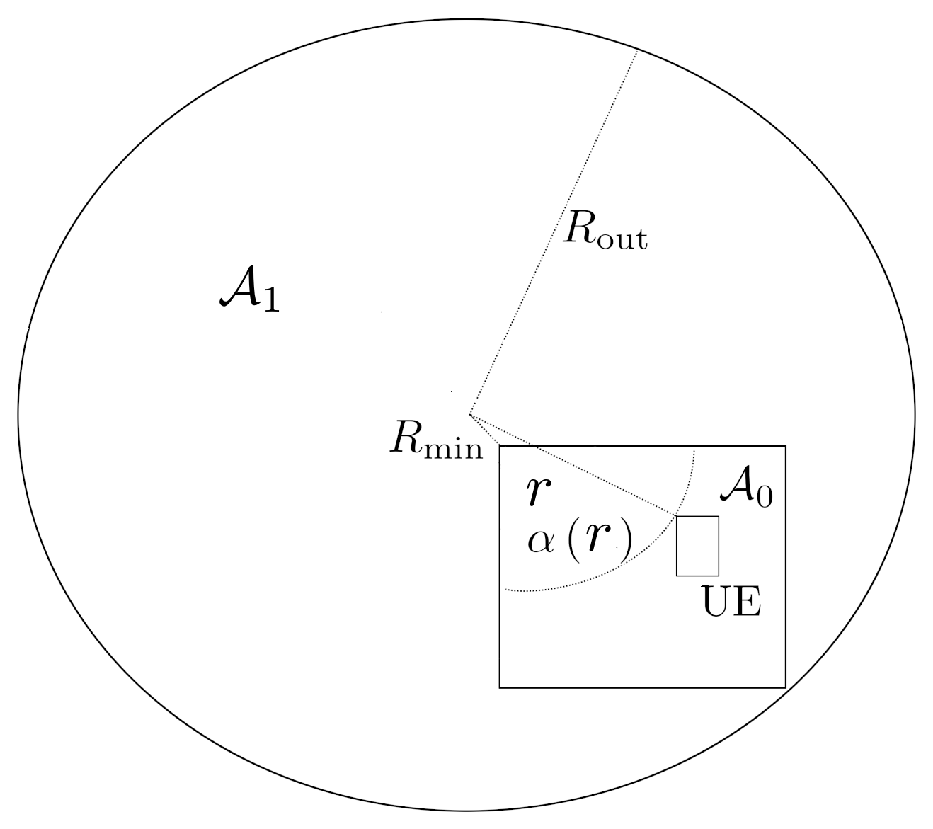
\includegraphics[width=0.5\columnwidth]{simpleScen.eps}
    \caption{Realization of the scenario over which \ac{np} hypothesis testing is performed: the \ac{ue} transmits message toward the \ac{bs} located at the center of the overall circular area. }
    \label{fig:scen}
\end{figure}

\subsection{Neural Network Implementation}\label{sec:nn}

Under more complicated scenarios, it becomes hard to obtain close-form expressions for the \ac{llr}. Therefore, we propose to use a \ac{ml} approach, where in the identification phase a \ac{nn} is trained with attenuation vectors $\bm{a}^{(i)}$ according to the labels $t_i \in \{0,1\}$. In the verification phase the \ac{nn} is used on the test attenuation vectors $\bm{y}$ to provide the decision $\hat{t} \in \{0,1\}$. We define $g(\cdot)$ to be the function implemented by the \ac{nn} such that
 \begin{equation}
 	\hat{t} = g(\bm{y}).	
 \end{equation}

A feed-forward \ac{nn} processes the input in stages, named layers, where the output of one layer is the input of the next layer. The input of the \ac{nn} is $\bm{y}^{(0)} = \bm{y}$, and layer $\ell-1$ has $N^{(\ell-1)}$ outputs obtained by processing the inputs with $N^{(\ell-1)}$ scalar functions named neurons. The output of the $n$-th neuron of the $\ell$-th layer is
\begin{equation}\label{eq:nonLin}
y_n^{(\ell)} = \sigma\left( \bm{w}_n^{(\ell -1)}\bm{y}^{(\ell-1)}+b_n^{(\ell)} \right),
\end{equation}
where $\bm{w}_n^{(\ell -1)}$ and $b_n^{(\ell)}$ are coefficients to be determined in the training phase, and $\sigma(\cdot)$ is the sigmoid activation function. 
%The neuron maps via  $\psi$ a  linear combination with weights $\bm{w}_n^{(\ell -1)}\in \mathbb{R}^{1\times N^{(\ell-1)}}$ of the outputs $\bm{y}^{(\ell-1)} \in \mathbb{R}^{N^{(\ell-1)} \times 1 }$ of the previous layer, plus a bias $b_n^{(\ell)} \in \mathbb{R}^{N^{(\ell-1)} \times 1 }$. 
The last layer comprises only one neuron, $y^{(L)}$, and the final output of the \ac{nn} is the scalar 
\begin{equation}
	\tilde{y} \triangleq \sigma(y^{(L)}),	
\end{equation}
where $L$ is the total number of layers. Finally, the test function is obtained by thresholding $\tilde{y}$, i.e.,
\begin{equation}
\label{eq:decNN}
    g(\bm{y}) = \begin{cases}
    1 & \tilde{y} > \lambda \\
    0 & \tilde{y} \leq \lambda.
    \end{cases}
\end{equation}
By varying $\lambda$ we obtain different values of $P_{\rm FA}$ and $P_{\rm MD}$ for this \ac{irlv} test.

Various options are considered in the literature for \ac{nn} training. We consider as objective function, the empirical \ac{ce} between the \ac{nn} output and the labels $t_i$ defined as
\begin{equation}\label{eq:ce}
\hatcross{\bm p_{\mathcal{H}|\bm y}}{g} \triangleq -\frac{1}{S} \sum_{i=1}^{S}\left[t_i\log \tilde{y}_i +\left(1-t_i\right)\log\left(1-\tilde{y}_i\right)\right],
\end{equation}
where $\tilde{y}_i = g(\bm a^{(i)})$, $i=1, \ldots, S$, is the soft output corresponding the $i^{\rm th}$  training point. Training is performed with gradient descent minimizing $\hatcross{\bm p_{\mathcal{H}|\bm y}}{g}$.

In the following we show that a \ac{ce} based \ac{nn} is equivalent, in probability and for perfect training, with the \ac{np} solution. First, we prove that the output of the \ac{nn} can be interpreted as the class conditional probability. 
\begin{theorem}
Let $\gy \in [0,1]$ be the output of a \ac{nn} obtained with perfect training, i.e., with infinite number of training points, layers and neurons. Then
\begin{equation}
	\gy = p(\mathcal{H}_0|\bm y)	
\end{equation}
almost surely.
\end{theorem}
\begin{proof}
Let $\bm y \in \mathcal{Y}$ be the input feature vector, where $|\mathcal{Y}|=S$. Consider then 
\begin{equation}
	\hatcross{\bm p_{\mathcal{H}|\bm y}}{g} = - \left[ \frac{n_0}{S} \frac{1}{n_0} \sum_{\bm y \in \mathcal{Y}_0} \log(\gy) 
		+ \frac{n_1}{S} \frac{1}{n_1} \sum_{\bm y \in \mathcal{Y}_1} \log(1-\gy) \right],	
\end{equation}
where $\mathcal{Y}_k = \{\bm y_i \in \mathcal{Y} : t_i = k\}$, $|\mathcal{Y}_k|=n_k$, $k \in \{0,1\}$.
Let $S \to \infty$. By the strong law of large numbers \cite{etemadi1981elementary}
\begin{equation}
\label{eq:as}
	\lim_{S \to \infty}	\hatcross{p_t}{\gy} = - \left[ p(\mathcal{H}_0) \int_{\mathcal{Y}} p(\bm y|\mathcal{H}_0) \log (\gy) d\bm y + 
		 p(\mathcal{H}_1) \int_{\mathcal{Y}} p(\bm y|\mathcal{H}_1) \log (1-\gy) d\bm y \right].
\end{equation}
Starting from \eqref{eq:as} included, all subsequent equalities are intended to hold in probability, i.e., \textit{almost surely}, as defined in the strong law of large number formulation.
Rearranging terms with the Bayes rule we get
\begin{equation}
\label{eq:dim1}
\lim_{S \to \infty}	\hatcross{\bm p_{\mathcal{H}|\bm y}}{g} = - \left\{ \int_{\mathcal{Y}} \bigl[ p(\mathcal{H}_0|\bm y) \log(\gy) + 
	(1-p(\mathcal{H}_0|\bm y)) \log(1-\gy)\bigr] p(\bm y)   d\bm y \right\}. 		
\end{equation}
We introduce the Bernoulli random variable $\xi$ with alphabet $ \{0,1\}$ and \ac{pdf} $\bm q = [q_0 \ q_1]$, where
\begin{subequations}
\label{eq:q}
\begin{align}
	q_0 &\triangleq \pr{\xi=0}=\gy \\
	q_1 &\triangleq \pr{\xi=1}=1-\gy.
\end{align}
\end{subequations}
Note that $\bm q$ is a valid \ac{pdf} since it sums to 1 and $\gy \in [0,1]$ by hypothesis. Let also 
\begin{equation}
	\bm p_{\mathcal{H}|\bm y} \triangleq [p(\mathcal{H}_0|\bm y)\ p(\mathcal{H}_1|\bm y)].	
\end{equation}
By definition of cross entropy and expected value, we have from \eqref{eq:dim1}
\begin{equation}
\label{eq:final}
	\lim_{S \to \infty}	\hatcross{\bm p_{\mathcal{H}|\bm y}}{g} =	\E{\bm y}{ \cross{\bm p_{\mathcal{H}|\bm y}}{\bm q}} = 
		\E{\bm y}{H (\bm p_{\mathcal{H}|\bm y}) + D(\bm p_{\mathcal{H}|\bm y}||\bm q)},
\end{equation}
where $D(\cdot||\cdot)$ is the Kullback-Leibler divergence, $H_{\bm c}(\bm d)$ is the cross entropy function between the two discrete \acp{pdf} $\bm c$ and $\bm d$, and $H(\cdot)$ is the entropy function. The second equality holds by definition of cross entropy.

Recall that \ac{nn} training is performed by minimizing \eqref{eq:final} with respect to \ac{nn} parameters. In the third term of \eqref{eq:final} the only quantity depending on \ac{nn} parameters, through $\gy$ in \eqref{eq:q}, is $D(\bm p_{\mathcal{H}|\bm y}||\bm q)$. The minimum is then attained for $D(\bm p_{\mathcal{H}|\bm y}||\bm q)=0$, that is when $\bm q = \bm p_{\mathcal{H}|\bm y}$.
\end{proof}

Note that this approach does not require the knowledge of the statistics of $\bm{y}$ under the two hypotheses, while, instead, it requires a large enough set of training points $S$ to converge.
However, at convergence, the \ac{nn} achieves the same performance of the NP approach. This holds since \eqref{eq:decNN} is equivalent to \eqref{eq:thrOpt}, i.e., they provide the same \ac{roc}, with
\begin{align}
	\tilde{y} &= p(\mathcal{H}_0|\bm y), \\
	\label{eq:relation}
	\theta &= \frac{1-\lambda}{\lambda} \frac{p(\mathcal{H}_0)}{p(\mathcal{H}_1)},	
\end{align}  
where \eqref{eq:relation} is a direct consequence of the Bayes rule applied as follows 
\begin{equation}
	p(\mathcal{H}_0| \bm y) = \frac{1}{1+  \frac{p(\mathcal{H}_1)}{p(\mathcal{H}_0)} \mathcal{L}^{(\bm y)}}.	
\end{equation}




% \subsection{Support Vector Machine}\label{sec:svm}
% A \ac{svm} \cite{Bishop2006} is a supervised learning model that can be used for classification and regression. We focus here on binary classification, i.e., we define the identification function as
% \begin{equation}
%   t_i =
%   \begin{cases}
%   -1 \quad \text{if} \quad \bm{y} \in \mathcal{A}_0\\
%   1 \quad \text{if} \quad \bm{y} \in \mathcal{A}_1.
%   \end{cases}
% \end{equation}
% Given the input vector $\bm{y}^{(0)} \in \mathbb{R}^N$ the \ac{svm} returns $\hat{t} = 1$ if $\bm{y}^{(0)}$ belongs to class 0 whereas $\hat{t}=-1$ if $\bm{y}^{(0)}$ belongs to class 1. It comprises the function $\tilde{t}: \mathbb{R}^N \to \mathbb{R}$ defined by
% \begin{equation}
% \label{eq:svm}
% \tilde{t} = \mathbf{w}^T \phi (\mathbf{a}^{(i)}) + b,
% \end{equation}
% where $\phi: \mathbb{R}^N \to \mathbb{R}^K$ is a feature-space transformation function, $\mathbf{w} \in \mathbb{R}^K$ is the weight vector and $b$ is a bias parameter, and the decision function is
% \begin{equation}
% \label{eq:cases}
% \hat{t} = 
% \begin{cases}
% +1 \quad \tilde{t}  \geq \gamma^* \\
% -1 \quad \tilde{t}  < \gamma^*,
% \end{cases}		
% \end{equation} 
% where $\gamma^*$ is a fixed threshold and controls \ac{fa} and \ac{md} probabilities. Note that in the classical \ac{svm} formulation we have $\gamma^* = 0$.

% While the feature-space transformation function is typically fixed, the vector $\mathbf{w}$ must be properly chosen to perform the desired classification


\section{Network Planning}\label{sec:bsPos}

As the attenuation depends on the position of the \acp{bs} and on the surrounding environment, the performance of the authentication system depends on the number of \acp{bs} and on their location. In this Section, we derive an approach to optimally locate \acp{bs} (\emph{network planning}) so that the authentication system attains the best performance. 


The optimal solution for \acp{bs} positioning in the \ac{irlv} context is given by the minimization of $P_{\rm MD}$ for each $P_{\rm FA}$ value, provided vy \ac{np}. We consider as performance metric the \ac{roc} curve, defined as the  function associating the $P_{\rm MD}$ with the corresponding $P_{\rm FA}$, for all possible values of thresholds $\lambda$. However, we do not want to fix {\em a priori} the value of $P_{\rm FA}$, but we instead want a single measure capturing the whole behaviour of the curve. We hence resort to the \ac{roc} \ac{auc} \cite{hanley-82}, defined as 
\begin{equation}
    K  = \int_{0}^{1} P_{\rm MD}\left(P_{\rm FA}\right) d P_{\rm FA},
\end{equation}
where $P_{\rm MD}\left(P_{\rm FA}\right)$ is the $P_{\rm MD}$ value as a function of $P_{\rm FA}$, which corresponds to the integral of the \ac{roc} function. Note that minimizing the \ac{auc}, is equivalent to minimize the average $P_{\rm MD}$ corresponding to a uniform $P_{\rm FA}$.
%\footnote{Notice that traditionally the \ac{auc} is a metric that needs to be maximized \cite{hanley-82}. This is due to the fact that the curve of the system performance computed as in \cite{hanley-82} and \cite{Kennedy-11} is given by the true positive rate vs. the false negative rate value, which is optimal when the true positive rate value is maximized for each false negative rate value. Since we consider as system performance metrics for the authentication system the $P_{\rm MD}$ and the $P_{\rm FA}$ we instead need to minimize the \ac{auc}.}
However, in order to compute the \ac{auc} we must run the \ac{nn} over a set of test attenuation vectors multiple times with different thresholds in order to estimate the \ac{roc} and compute numerically its integral.

We hence propose to exploit the training process of the \ac{nn} and use the \ac{ce}, readily provided at the end of training, as a proxy of the system performance, so that we don't need to estimate the \ac{roc} and compute the \ac{auc}. This is motivated by Theorem 1 as the lower \ac{ce}, the more a \ac{nn} approaches \ac{np}, which is the optimal solution. 
Recalling that the training minimization problem is non-convex, the same training set can lead to \acp{nn} with different classification performance and hence different \ac{auc}. However we keep the one with minimum \ac{ce}, which is expected to have the minimum \ac{auc}.


 
% Since $t$ and $\hat{t}$ are Bernoulli variables, the \ac{kl} between $t$ and $\hat{t}$ can be written as 
%\begin{equation}
%\mathbb D(p_t; p_{\hat{t}}) = P_{\rm MD} \log \frac{P_{\rm MD}}{1 - P_{\rm FA}} + (1-P_{\rm MD})\log \frac{1- P_{\rm MD}}{P_{\rm FA}}\,,
%\label{KLb}
%\end{equation}
%where $p_t$ is the \ac{pmd} of $t$, $p_{\hat{t}}$ is the \ac{pmd} of $\hat{t}$. Now, since $\hat{t}$ is obtained by $\tilde{y}$, by the data processing inequality we have (see also \cite{Tomasin-Ferrante}) that {\em for any thresholding of $\tilde{y}$}
%\begin{equation}
%\mathbb D(p_t; p_{\hat{t}}) \leq \mathbb D(p_t; p_{\tilde{y}})\,.
%\label{dpi}
%\end{equation}
%Therefore, the right term of the inequality is  a synthetic metric of the test, irrespective of the optimization of the threshold, i.e., of a specific target \ac{fa} probability. The \ac{auc} is also another synthetic description irrespective of the specific thresholding. Now let us establish the connection between \ac{fa} and \ac{md} probabilities and \ac{ce}. The \ac{ce} used for \ac{nn} optimization (\ref{eq:ce})  can also written as 
%\begin{equation}
%\mathbb H(p_t,p_{\tilde{y}}) = \mathbb H(p_t) +\mathbb D(p_t; p_{\tilde{y}})\,,
%\end{equation}
%where $\mathbb H(\cdot)$ is the entropy function and $\mathbb D(\cdot;\cdot)$ is the \ac{kl} divergence. Therefore by  adding $\mathbb H(p_t)$ to both terms in (\ref{dpi}) we have 
%\begin{equation}
%\mathbb H(p_t) +\mathbb  D(p_t; p_{\hat{t}}) \leq \mathbb H(p_t,p_{\tilde{y}})\,. 
%\end{equation}
%Since the entropy of $t$ is the same for all testing techniques, minimizing the \ac{ce} is equivalent to minimizing an upper bound on the \ac{kl} divergence between $t$ and $\hat{t}$, which can be written as a function of \ac{fa} and \ac{md} probabilities by (\ref{KLb}). This justifies the use of the \ac{ce} as a metric for the optimization of the \ac{bs} position.

\subsection{Particle Swarm Optimization}

As before stated, the training algorithm is not convex, and neither it is the network planning \ac{auc} minimization problem. In order to solve the \acp{bs} positioning problem we exploit the \ac{pso} \cite{Kennedy-11}, which is an iterative algorithm performing the simultaneous optimization of different points. This is similar to the multi-start solution for non-convex optimization, where local minima are avoided by selecting among different descent paths the one providing the minimum solution. The \ac{pso} is briefly recalled here.
 
\ac{pso} is an iterative optimization algorithm based on social behavior of animals, e.g., birds flocking and fish schools. Consider a total number $P$ of particles, where  particle $p=1, \ldots P$, is described by a vector of \acp{bs} positions $\bm{x}_p = [\bm{x}_{\rm ap}^{(1)}(p),\ldots, \bm{x}_{\rm ap}^{(N_{\rm ap})}(p)]$ and by its velocity $\bm{v}_p$.  Each particle is a candidate solution of the optimization problem. Starting from a random position for all the particles, at each iteration both  positions $\bm{x}_p$ and  velocities $\bm{v}_p$ are updated. Two optimal values are defined in each iteration: the global optimum found so far by the entire population and a local optimum for each particle, i.e., the optimal value found by the individual $p$ up to the current iteration. We define as $\bm{o}_g$ the position of the the global optimal values and as $\bm{o}_p$ the position of the optimal value found by particle $p$ at the current iteration. The optimal values are those minimizing the selected objective function.

The position and velocity of the particles are updated at iteration $\ell$ as \cite{Kennedy-11}
   \begin{equation}\label{eq: v up}
\begin{split}
  \bm{v}_p(\ell) = \omega \bm{v}_p(\ell-1)+\phi_1(\ell)(\bm{o}_p(\ell-1)-\\
  -\bm{x}_p(\ell-1))+\phi_2(\ell)(\bm{o}_g(\ell-1)-\bm{x}_p(\ell-1));
  \end{split}
  \end{equation}
  \begin{equation}\label{eq: p up}
  \bm{x}_p(\ell) = \bm{x}_p(\ell-1) + \bm{v}_p(\ell);
 \end{equation}
where $\omega$ is the inertia coefficient and $\phi_1$ and $\phi_2$ are random variables uniformly distributed in $[0,c_1]$ and $[0,c_2]$, respectively, where $c_1$ and $c_2$ are defined as acceleration constants. The values of the inertia coefficient and of the acceleration constants are the parameters of the \ac{pso} problem.

\subsection{PSO-Based Network Planning}

As we have seen the \ac{roc} \ac{auc} well describes the overall behaviour of the \ac{roc} and is hence widely recognized as a valid synthetic metric for hypothesis testing. On the other hand, computation of the \ac{auc} is complicated by the need of performing extensive testing, while the \ac{ce} is immediately provided after the \ac{nn} training process. 

In particular, the testing needed to compute \ac{auc} has an additional complexity (with respect to training that must be performed anyway), of 
\begin{equation}
    \mathcal{C}_{\rm test} = P \left( \mathcal{C}_{\rm out}+\mathcal{C}_{\rm ROC}+\mathcal{C}_{\rm AUC}\right),
\end{equation}
where  $\mathcal{C}_{\rm out}$ denotes the complexity associated to running the \ac{nn} on the test points, $\mathcal{C}_{\rm ROC}$ denotes the complexity of building the \ac{roc} function and $\mathcal{C}_{\rm AUC}$ denotes the complexity of integrating the \ac{roc}. The \ac{nn} running cost $\mathcal{C}_{\rm out}$ is given by the total number of multiplication and additions needed to compute the output value $y^{(L-1)}$ for all testing vectors, i.e.,
\begin{equation}
    \mathcal{C}_{\rm out} = \left(2N_{\rm AP}N_{\rm h}+2N_{\rm h}^2N_{\rm L} + 2N_{\rm h}\right)\tau ,
\end{equation}
where $N_{\rm h}$ is the number of neurons in the hidden layer, $N_{\rm L}$ is the number of hidden layers and $\tau$ is the size of the testing set.
The computation of the \ac{roc} curve requires the estimation of the $P_{\rm FA}$ and $P_{\rm MD}$ values for each threshold value $\lambda$, whereas the computation of the \ac{auc} requires the numerical integration of the \ac{roc} curve over $P_{\rm FA}$ values.

The proposed \ac{pso}-based network planning algorithm is reported in Algorithm 1. We denote as $\mathcal{B}$ the optimization metric and we initialize $P$ particles with random positions for each of the $N_{\rm AP}$ \acp{bs} in each particle. For each particle we train the \ac{nn} and compute $\mathcal{B}_p^{(0)}$. The global optimum value $\mathcal{B}_g$ is set to the minimum among all $\mathcal{B}_p^{(0)}$ values. Then, positions and velocities of the particles are updated via (\ref{eq: v up}) and (\ref{eq: p up}), and both the local and global optimum are updated according to the obtained values at the current iterations. The algorithm stops when the global optimum converges.

 \begin{algorithm}[b!]

\small

  \KwData{ number of particles $P$, $N_{\rm AP}$}
  \KwResult{optimal position }
  Initialize particles\;
  train the \ac{nn} algorithm for each particle\;
  $\mathcal{B}_p^{(0)}$, $p=1,...,N_p$\;
  $\mathcal{B}_g=\underset{p=1,...,N_p}{min} \, \mathcal{B}_p^{(0)}$\;
  $i = 0$\;

  \Repeat{convergence of $\mathcal{B}_g$}{
         $i = i + 1$\;
         \For{$p=1,\ldots,P$}{
         update velocity and position vector of particle via (\ref{eq: v up}) and (\ref{eq: p up})\;
                  train the \ac{nn} for each particle $\to$ $\mathcal{B}_p^{(i)}$\;
                  \If{$\mathcal{B}_p^{(i)} < \mathcal{B}_g$}{ $\mathcal{B}_g = \mathcal{B}_p^{(i)}$ \;}
         }
      
      }
      
\caption{Proposed \ac{ce}-based APs positioning algorithm.}
 \end{algorithm}      

%  \begin{algorithm}[b!]

% \small

%   \KwData{ number of particles $P$, $N_{\rm AP}$}
%   \KwResult{optimal position }
%   Initialize particles\;      
%       train the \ac{nn} algorithm for each particle $\to$ $K_p^{(0)}$, $p=1,...,N_p$\;
%   $K_g=\underset{p=1,...,N_p}{min} \, K_p^{(0)}$\;
%       $i = 0$\;
%       \Repeat{convergence of $K_g$}{
%          $i = i + 1$\;
%          \For{$p=1,\ldots,P$}{
%          update velocity and position vector of particle via (\ref{eq: v up}) and (\ref{eq: p up})\;
%                   train the \ac{nn} for each particle \;
%                   test the \ac{nn} $\to$
%                   $K_p^{(i)}$\;
%                   \If{$K_p^{(i)} < K_g$}{ $K_g = K_p^{(i)}$ \;}
%          }
      
%       }
    
% \caption{Proposed \ac{auc}-based APs positioning algorithm.}
%  \end{algorithm}

Notice that, as the optimization problem is non-convex, solving \ac{pso} is similar to a multi-start optimization considering $P$ different starting points, which is a standard method used to avoid local minimum solutions. As the number $P$ increases the probability of resolving to a local solution is reduced.

\section{Numerical Results}\label{sec: nr}

We first compare the \ac{nn} solution with the optimal \ac{np} test in the \ac{los} scenario, using a single \ac{bs} as described in Section \ref{sec:los}. We consider a \ac{nn} with $N_L=3$ hidden layers and different number $N_h$ of neurons in the hidden layer. Training and testing have been performed with $10^6$ points each. 

Fig. \ref{fig:NP_comp} shows the \ac{roc} obtained with the \ac{np} test and with the \ac{nn}. We see that, even with a small number of neurons, in this simple problem, the \ac{nn} achieves the same \ac{roc} of the \ac{np} test. This is a numerical demonstration of Theorem 1.

 
 \begin{figure}[h]
     \centering
     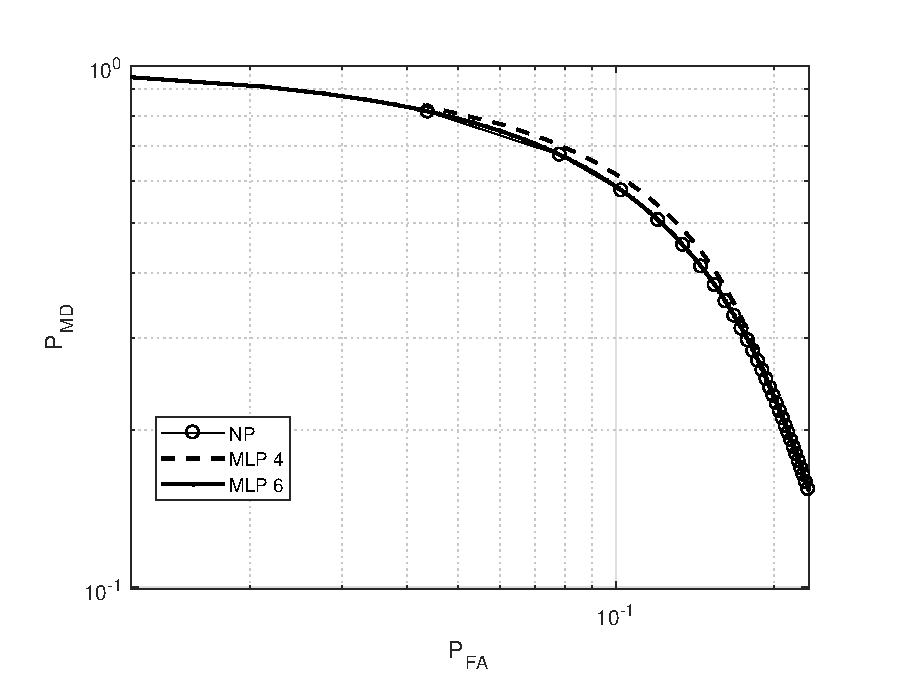
\includegraphics[width=0.9\columnwidth]{FA_MD_LOS.eps}
     \caption{\ac{roc} of the \ac{np} test and the the proposed \ac{ml} test,  with different number of neurons in the hidden layer of the \ac{nn}.}
     \label{fig:NP_comp}
 \end{figure}

 
In order to test the \ac{nn} approach in a more challenging scenario, we consider a network with $N_{\rm AP}=5$ \acp{bs}, each  characterized by a different  shadowing map, obtained with the model described in Section II, for a square area with two streets dividing the square into four quadrants with buildings, and the safe area $\mathcal A_0$  located in a quadrant, inside the building.

%Fig. \ref{fig:trueMap} shows a realization of the path loss and shadowing map for an \ac{bs} located in the center of the area $\mathcal{A}$. 
%We further assume that inside $\mathcal{A}$ there are  two orthogonal \ac{los} paths traversing the center of $\mathcal{A}$, representing for example streets surrounded by buildings. We indicate region $\mathcal A_0$   by the red line.


% \begin{figure}[t]
%     \centering
%     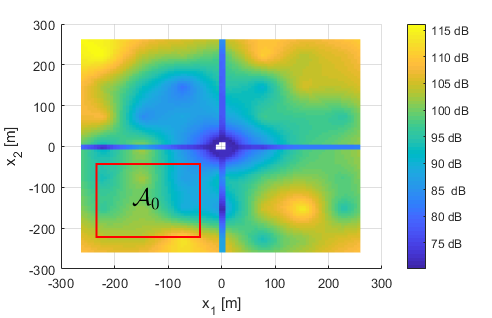
\includegraphics[width=0.9\columnwidth]{surfColorato.png}
%     \caption{Example of a realization of the attenuation map in the non-\ac{los} scenario considering only the shadowing effects.}
%     \label{fig:trueMap}
% \end{figure}

Fig. \ref{fig:n_train} shows the average (over shadowing realizations) \ac{roc} of the proposed \ac{nn} \ac{irlv} system  trained with different number of training points $q$. Results have been obtained for a $N_L=3$ layer \ac{nn} with $N_h=5$ neurons in the hidden layer. We see that the \ac{auc} decreases when increasing the number of training points and that, starting from $q=10^6$, the \ac{roc} does not improve. This is due to the the fact that, for the selected \ac{nn} architecture, training has reached convergence and hence adding further data to the training process does not add information to the function implemented by the \ac{nn}. 

\begin{figure}[t]
    \centering
    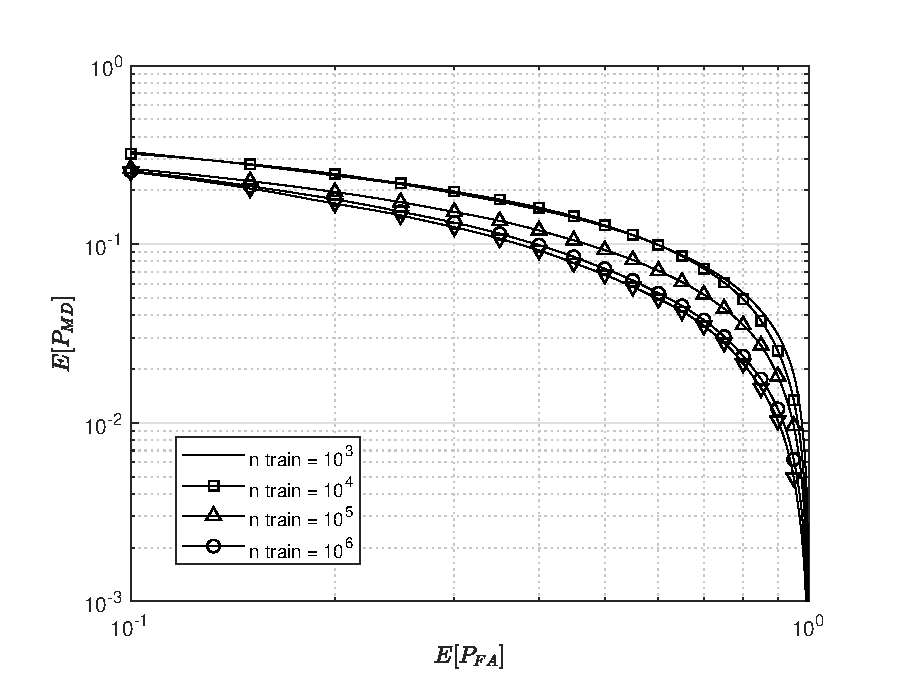
\includegraphics[width=0.9\columnwidth]{mean_maps_2.eps}
    \caption{\ac{roc} of the \ac{nn} \ac{irlv} system trained with $q$ training points.}
    \label{fig:n_train}
\end{figure}

\subsection{Network Planning Performance}

We consider now the network planning using the proposed Algorithm 1. We consider a \ac{pso} with $P=6$ particles, each composed by a set of $N_{\rm AP}=5$ \acp{bs} initialized with random positions. There exists a variety of implementations of the \ac{pso}, but the most general case for the parameters initialization is given by \cite{clerc2002}, i.e.,   $\omega=0.7298$, $c_1=c_2=1.4961$. Results are averaged over different shadowing realizations. We consider $10^4$ training  points and  $10^3$ testing points. In order to validate the use of the \ac{ce} as a proxy for the \ac{auc}, we compare the performance of Algorithm 1 using $\mathcal{B}=$\ac{ce} and using $\mathcal{B}=$\ac{auc}. The overall performance metric is the \ac{auc}.

Fig. \ref{fig:CEvsAUC} shows the average \ac{auc} value vs. the number of \ac{pso} iterations. We see that the \ac{ce}-based solution reaches approximately the same  \ac{auc} value of the \ac{auc}-based solution as the number of iterations increases. 
Note that the result of Theorem 1 holds asymptotically and with perfect training (in terms of training set, number of layers and neurons), which are conditions that our experiments do not satisfy. This explains the following two observations. The former is that there is a  difference between the \ac{auc} convergence values for the two algorithms. However, this difference is small ($\sim 10^{-4}$). The latter is that the \ac{auc}-based algorithm converges earlier, at iteration 3, than the \ac{ce}-based algorithm, at iteration 5. This last point can be explained by the fact that full convergence has not been reached by the \ac{nn} due to the finite number of neurons and samples in the training set. Therefore the obtained \ac{ce} is an approximation of the selected objective function, requiring more gradient descent steps than those required by the direct optimization of the \ac{auc}.   

%Fig. \ref{fig:CEvsAUC} shows the average \ac{auc} value vs. the number of \ac{pso} iterations. We see that the \ac{ce}-based solution reaches approximately the same  \ac{auc} value of the \ac{auc}-based solution as the number of iterations increases. Recalling that \eqref{eq:final} is obtained as asymptotic result, the fact that the \ac{ce} based solution requires a larger number of iteration to reach the minimum is due to the fact that results obtained by simulations consider finite number of neurons and finite training set. However we notice that also in the finite case the \ac{ce} minimization provides a good approximation of the classification performance of the network.

 
% Fig. \ref{fig:cdf} shows the \ac{cdf} of the number of  iterations using \ac{ce} as objective function in Algorithm 1. We note that in half of the cases only four iterations are performed using \ac{ce} and then the rest of the iterations are using the \ac{auc} as a target function. Since from Fig. \ref{fig:CEvsAUC} we note that in five  iterations Algorithm 1 is on average already quite close to convergence we can conclude that the number of iterations in the \ac{auc} stage is very small in most cases. This does not occur for the pure \ac{auc} solution, where a higher number of \ac{auc} iterations is needed to achieve convergence (see  Fig. \ref{fig:CEvsAUC}).
%\balance
\begin{figure} 
    \centering
    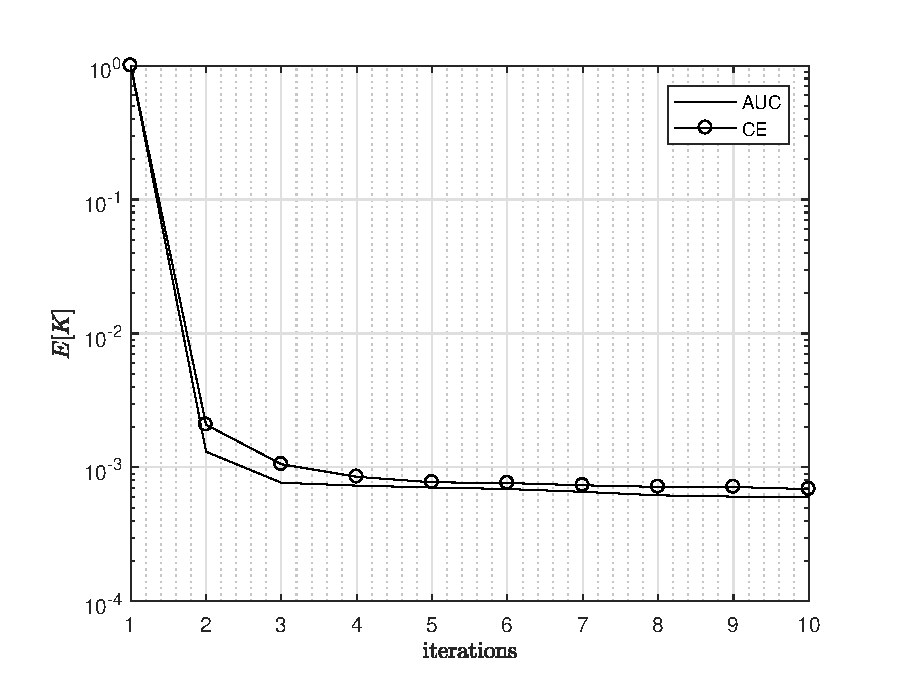
\includegraphics[width=0.9\columnwidth]{newPSO.eps}
    \caption{Mean \ac{auc} vs. the number of \ac{pso} iterations for Algorithm 1, and two \ac{pso} algorithms using only the  \ac{auc} and the \ac{ce} as objective functions. }
    \label{fig:CEvsAUC}
\end{figure}

% \begin{figure} 
%     \centering
%     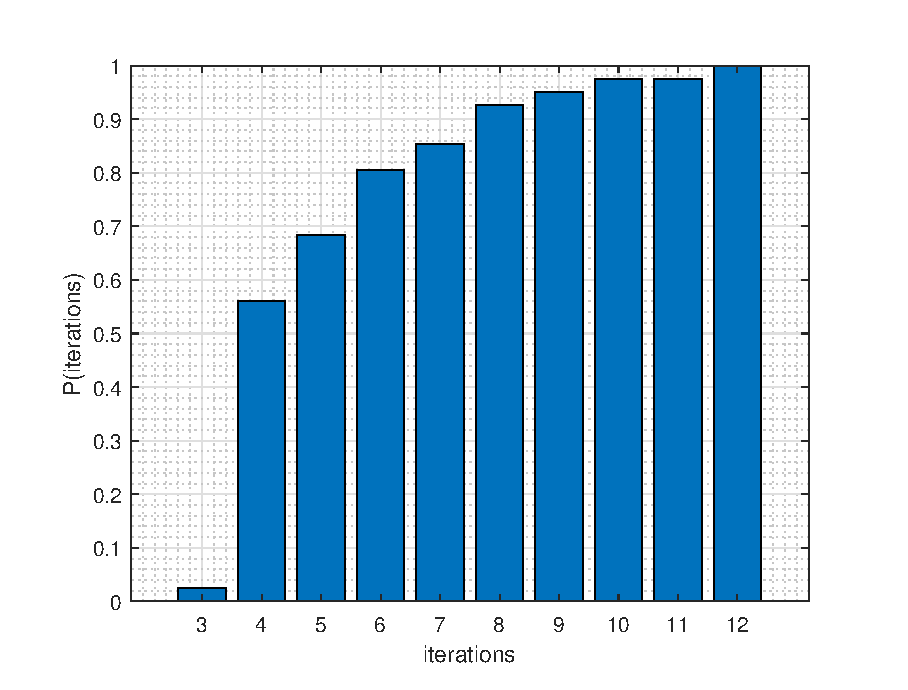
\includegraphics[width=0.9\columnwidth]{cdf_bar.eps}
%     \caption{CDF of the number of iterations of the first stage of Algorithm 1. }
%     \label{fig:cdf}
% \end{figure}
 
\section{Conclusions}
\label{sec:conc}
%\balance

In this paper we formulated the \ac{irlv} problem as an hypothesis testing problem and proposed a \ac{ml} solution. We proved that the \ac{nn} implementation achieves the same performance of the optimal \ac{np} test and verified numerically this claim for a simple scenario. We also assessed the effects of the training set size over the \ac{roc} for a more complicated scenario. We then proposed a \ac{pso}  algorithm for the  optimal \acp{bs} positioning, establishing the connection of two objective functions, \ac{ce} and \ac{auc}, in terms of  \ac{roc}.
% We then showed by numerical results the effectiveness of the proposed solution in terms of \ac{auc} of the \ac{roc}.


\renewcommand*{\bibfont}{\footnotesize}

\printbibliography

\end{document}
